%! Author = noone
%! Date = 8/10/22

% Preamble
\documentclass[11pt]{article}
\documentclass{beamer}

% Packages
\usepackage{amsmath}
\usepackage{graphicx}
\usepackage{float}
\usepackage{multimedia}
\usepackage{blindtext}
\usepackage{hyperref}

% Document
\begin{document}

\section{Week 4: Overview}\label{sec:week-4:-overview}

    This week, we will explore the use of neural networks for sequence and language processing.
Simple Recurrent Networks (SRN) can be trained to recognize or predict formal languages, and we can analyse their hidden unit dynamics.
By the use of a gating mechanism, Long Short Term Memory (LSTM) and Gated Recurrent Networks (GRU) are able to learn longer range dependencies than SRN.

Then we will look at the statistics of language, and show how word vectors can be assigned in a systematic way using approximations to singular value decomposition such as word2vec and GloVe.

\section{Weekly learning outcomes}\label{sec:weekly-learning-outcomes}

By the end of this week, you will be able to:
- design and train neural networks for processing temporal sequences
- describe different architectures including sliding windows, simple recurrent networks, Long-Short Term Memory (LSTM), and Gated Recurrent Units (GRU)
- analyse hidden unit dynamics of recurrent networks
- describe word frequencies, n-gram model, co-occurrence matrix
- describe the components and properties of singular value decomposition
- describe the word2vec model, including architecture, cost function and efficiency issues

\section{Recurrent Networks}
\section{Processing Temporal Sequences}

There are many tasks for which the output depends on a sequence of inputs rather than a single input.
For example:
- speech recognition
- time series prediction
- machine translation
- handwriting recognition
- How can neural network models be adapted for these tasks?

\section{NetTalk sliding window approach}

The simplest way to process temporal sequences using a neural network is the *sliding window* approach, first used in the NetTalk system (Sejnowski and Rosenberg, 1987).
English text is fed to NetTalk as a sequence of characters, and it outputs a sequence of phonemes indicating how that text should be pronounced.
Specifically, its input consists of seven consecutive characters and it aims to output a set of phonetic attributes specifying the correct pronunciation for the middle character.
In order to illustrate why it is necessary to know a few characters to the left and right of the middle character, consider how the first vowel would be pronounced in each of the following examples:
- pa, pat, pate, paternal
- mo, mod, mode, modern.

\begin{figure}
    \centering
    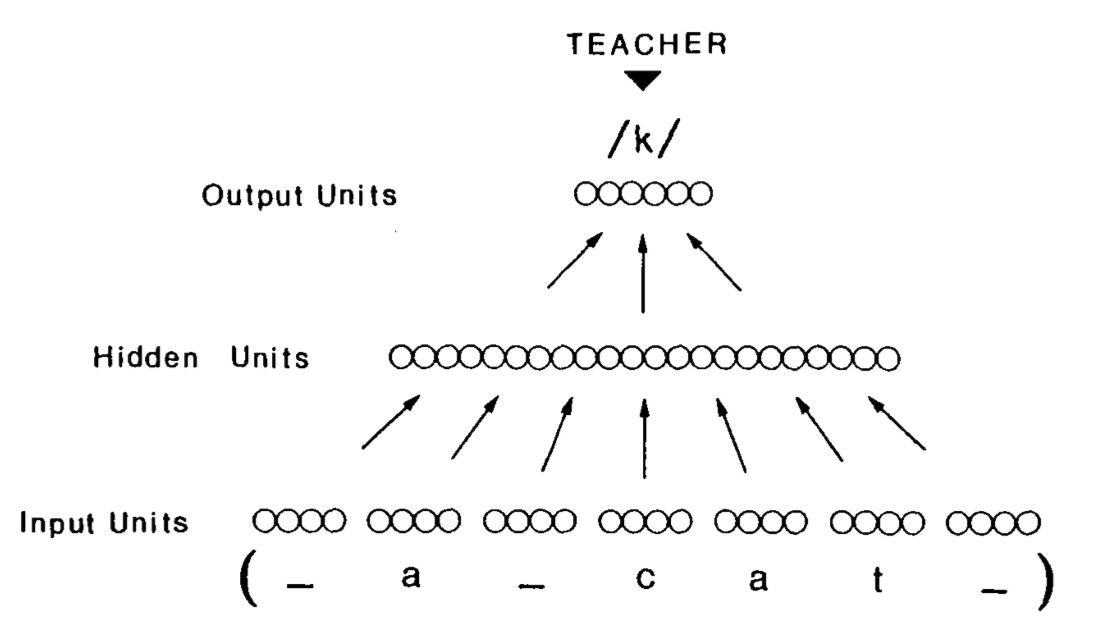
\includegraphics[width=12cm, height=8cm]{/home/noone/Documents/GitHub/neural_networks/out/images/recurrent-networks}
    \caption[recurrent networks]{recurrent networks}
    \label{fig: recurrent networks}
\end{figure}

For each of the seven input characters, a one-hot encoding is used with 29 units (including the 26 letters, plus punctuation and word boundaries) making a total of 203 inputs.
There were 80 hidden units with sigmoidal transfer function, and 26 outputs encoding 21 articulatory features plus stress and syllable boundaries.

NetTalk gained a lot of media attention at the time, partly because the output was hooked up to a speech synthesiser.
In the early stages of training, it sounds a bit like a babbling baby.
When fully trained, it sounds reasonable, although somewhat robotic.

\frame{
    \frametitle{Embedded Video}
    \begin{center}
        \movie{\includegraphics[width=\textwidth]{}}{w4_language_processing/NETtalk Test.mp4}
    \end{center}
}

Critics have sometimes claimed that a decision tree could produce equally good or better accuracy.
In any case, this kind of approach can only learn short-term dependencies, not the medium or long-term dependencies that are required for some tasks.

\section{Simple Recurrent Network}\label{sec:simple-recurrent-network}

\begin{figure}[h]
    \centering
    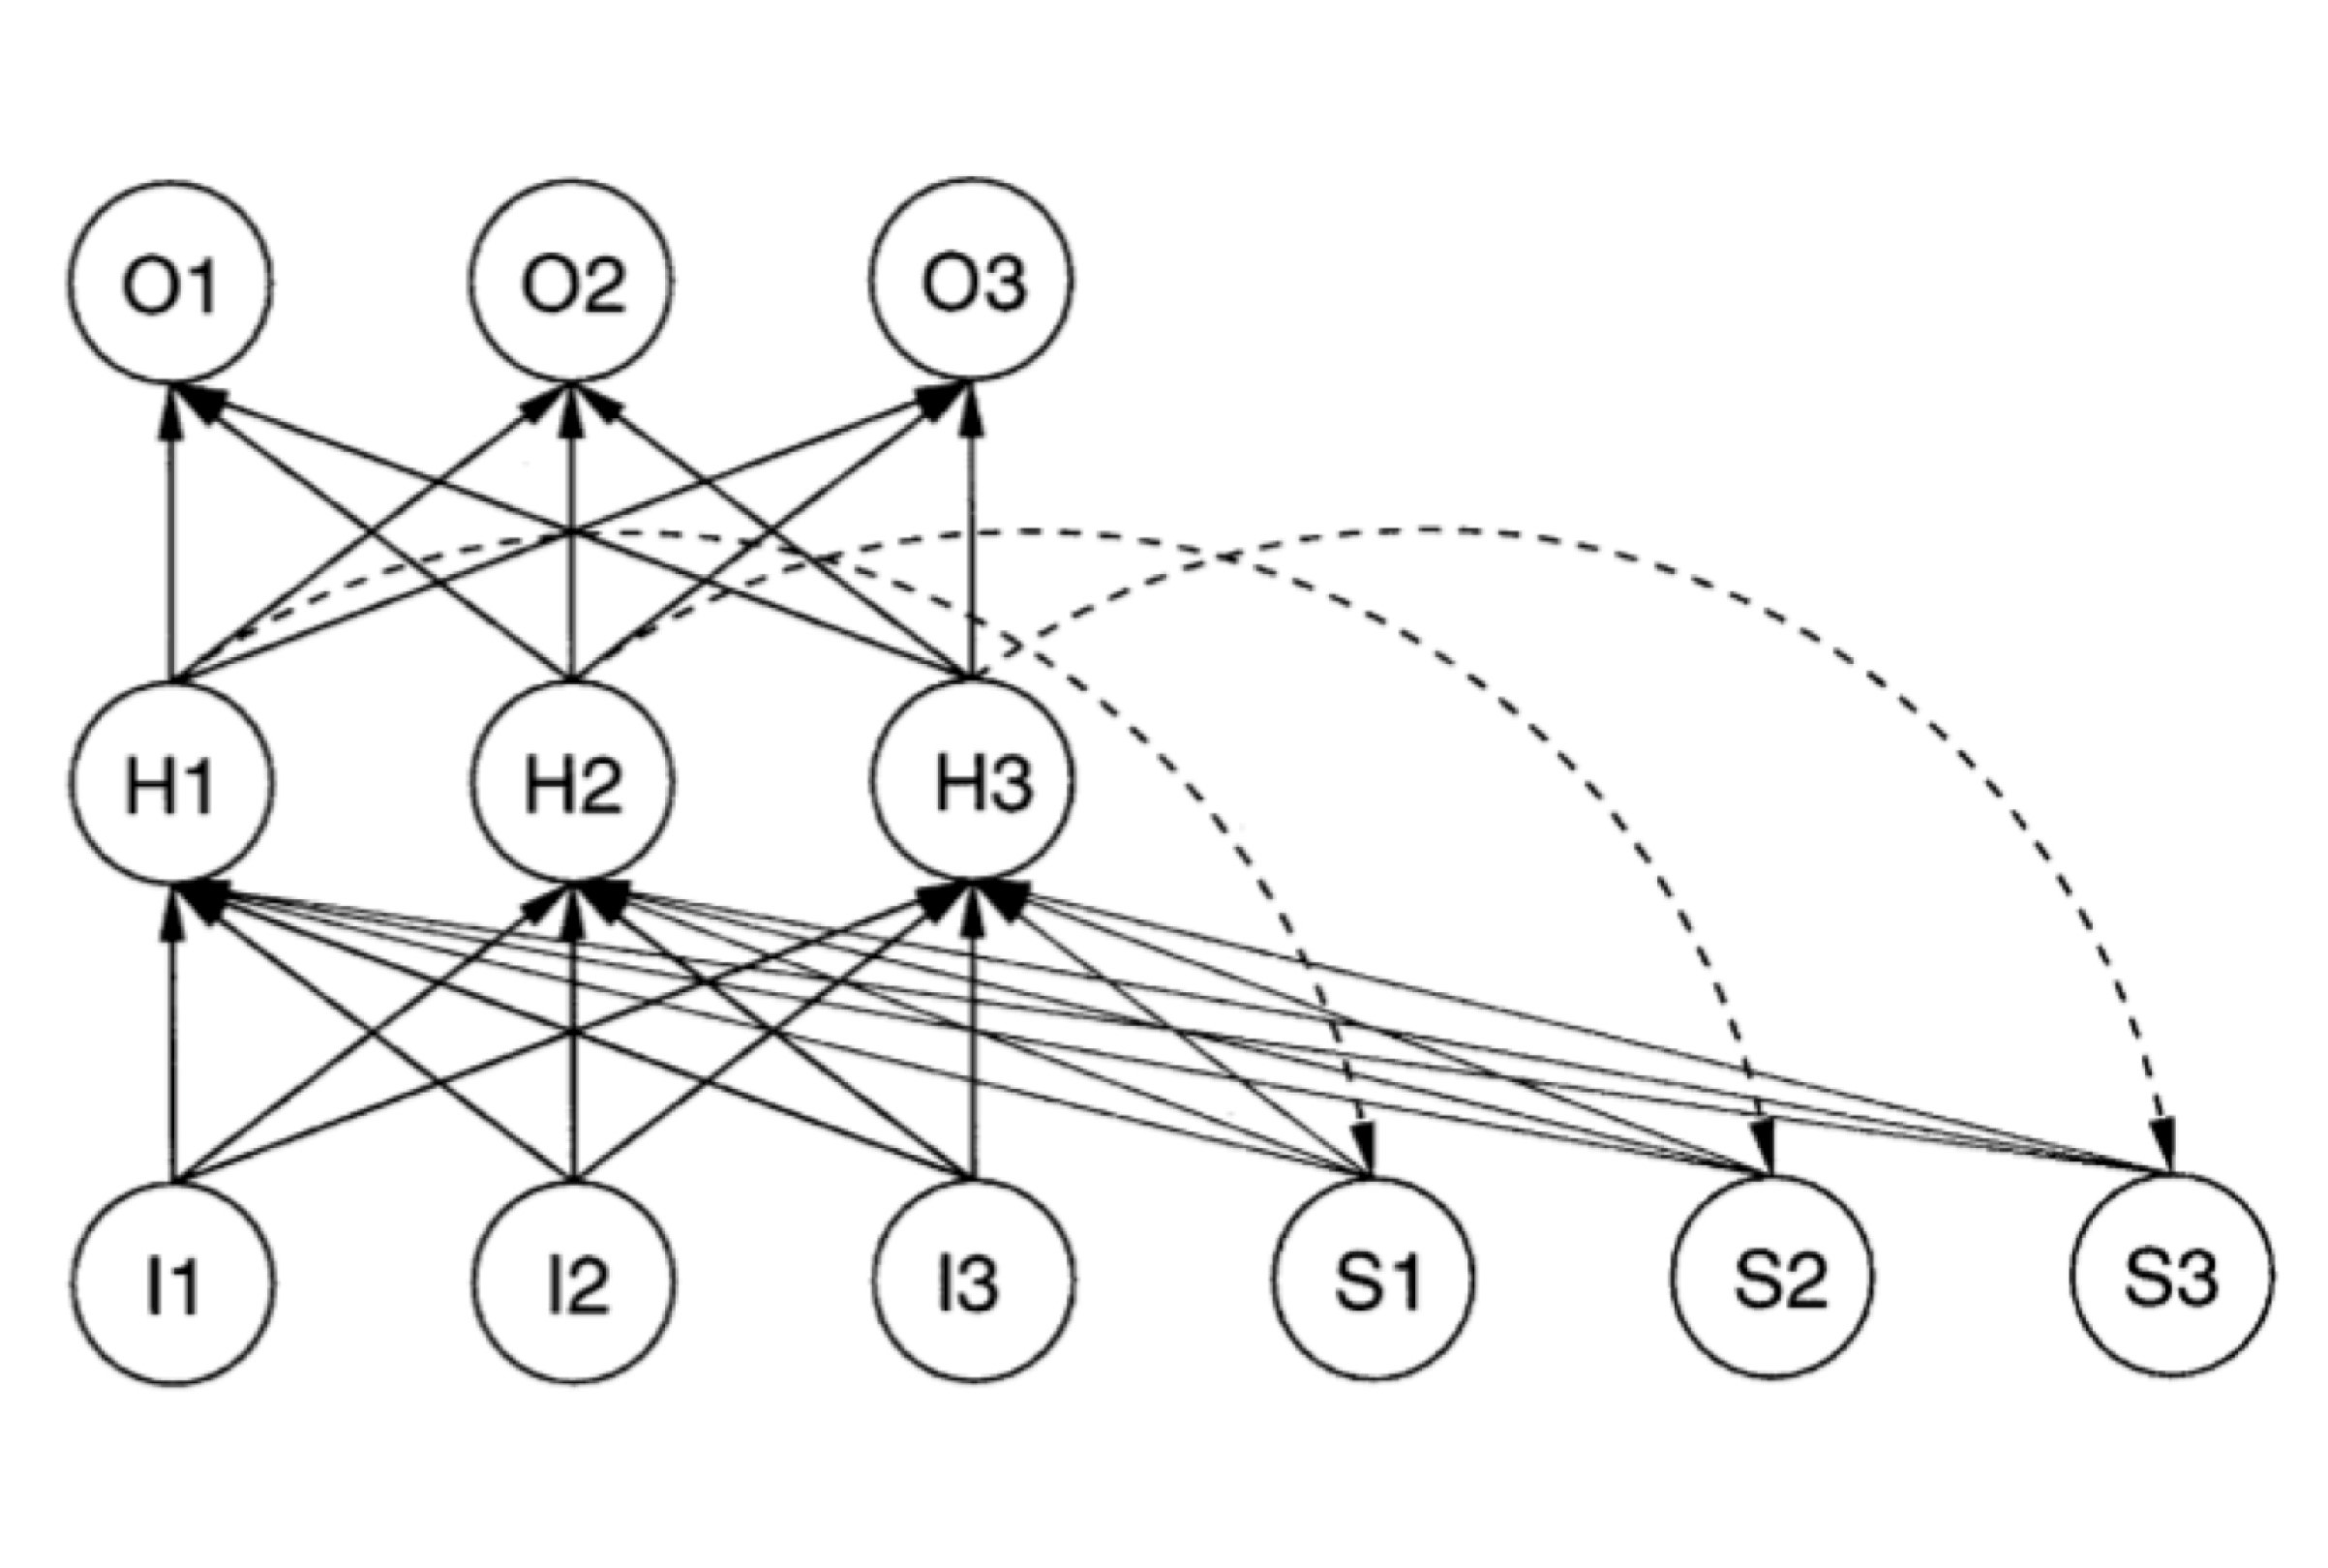
\includegraphics[width=8cm, height=7cm]{/home/noone/Documents/GitHub/neural_networks/out/images/simple-recurrent-network}
    \caption[simple recurrent network]{simple recurrent network}
    \label{fig: simple recurrent network}
\end{figure}

Simple Recurrent Networks (SRN) were introduced in Elman (1990).
A sequence of inputs are fed to the network one at a time.
At each timestep, the current activations in the hidden layer are copied to a *context* layer.
The new activations for the hidden layer are then calculated from the current input and the context layer.
Thus, the context layer is used to *remember* whatever information the network requires in order to predict the correct output.

The basic SRN can be augmented with *shortcut* connections directly from input to output, or connections from the output back to the hidden layer (sometimes called “Jordan Networks”).

\section{Backpropagation Through Time}\label{sec:backpropagation-through-time}

For any given input sequence, we can *unroll* a recurrent architecture into an equivalent feedforward architecture, with shared weights.
Applying backpropagation to the unrolled architecture is referred to as **backpropagation through time**.
We can backpropagate just one timestep, or a fixed number of timesteps, or all the way back to the beginning of the sequence.

\begin{figure}[h]
    \centering
    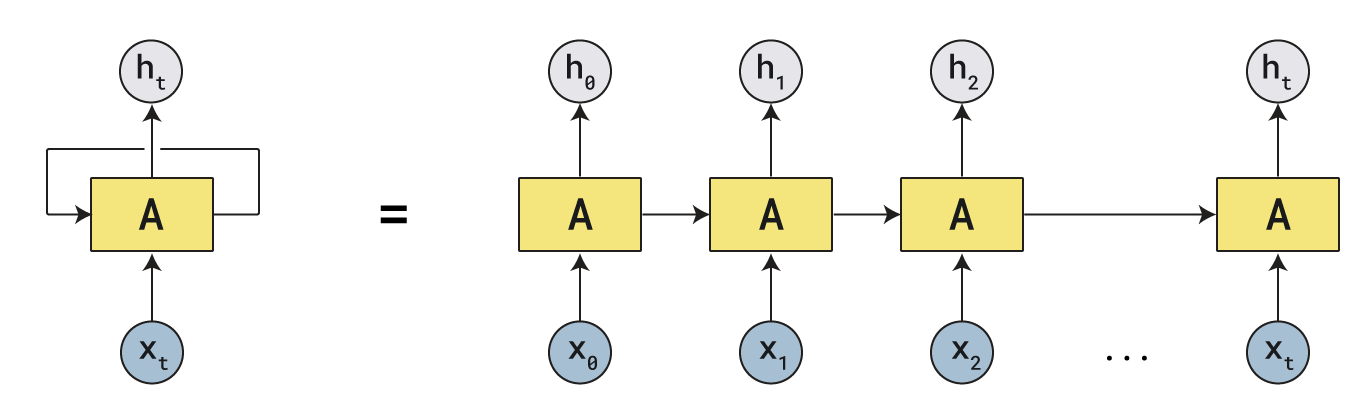
\includegraphics[width=12cm, height=8cm]{/home/noone/Documents/GitHub/neural_networks/out/images/back-propagation-through-time}
    \caption[back propagation through time]{back propagation through time}
    \label{fig: back propagation through time}
\end{figure}

\href{http://colah.github.io/posts/2015-08-Understanding-LSTMs/}{Understanding LSTMs}

insert video

\section{Recognizers and Predictors}\label{sec:recognizers-and-predictors}

    The basic SRN can be augmented with *shortcut* connections directly from input
to output, or connections from the output back to the hidden layer (sometimes
called “Jordan Networks”).
Another architecture which has been explored for binary sequences is the Second
Order Network or Gated Network, where the input symbol ($$0$ or $1$$) is used
to choose between two sets of weights $W_0$ and $W_1$.
The weights $W0$, $W_1$ and $P$ and the initial state $x_0$ can all be trained
by backpropagation through time.

\begin{figure}[h]
    \centering
    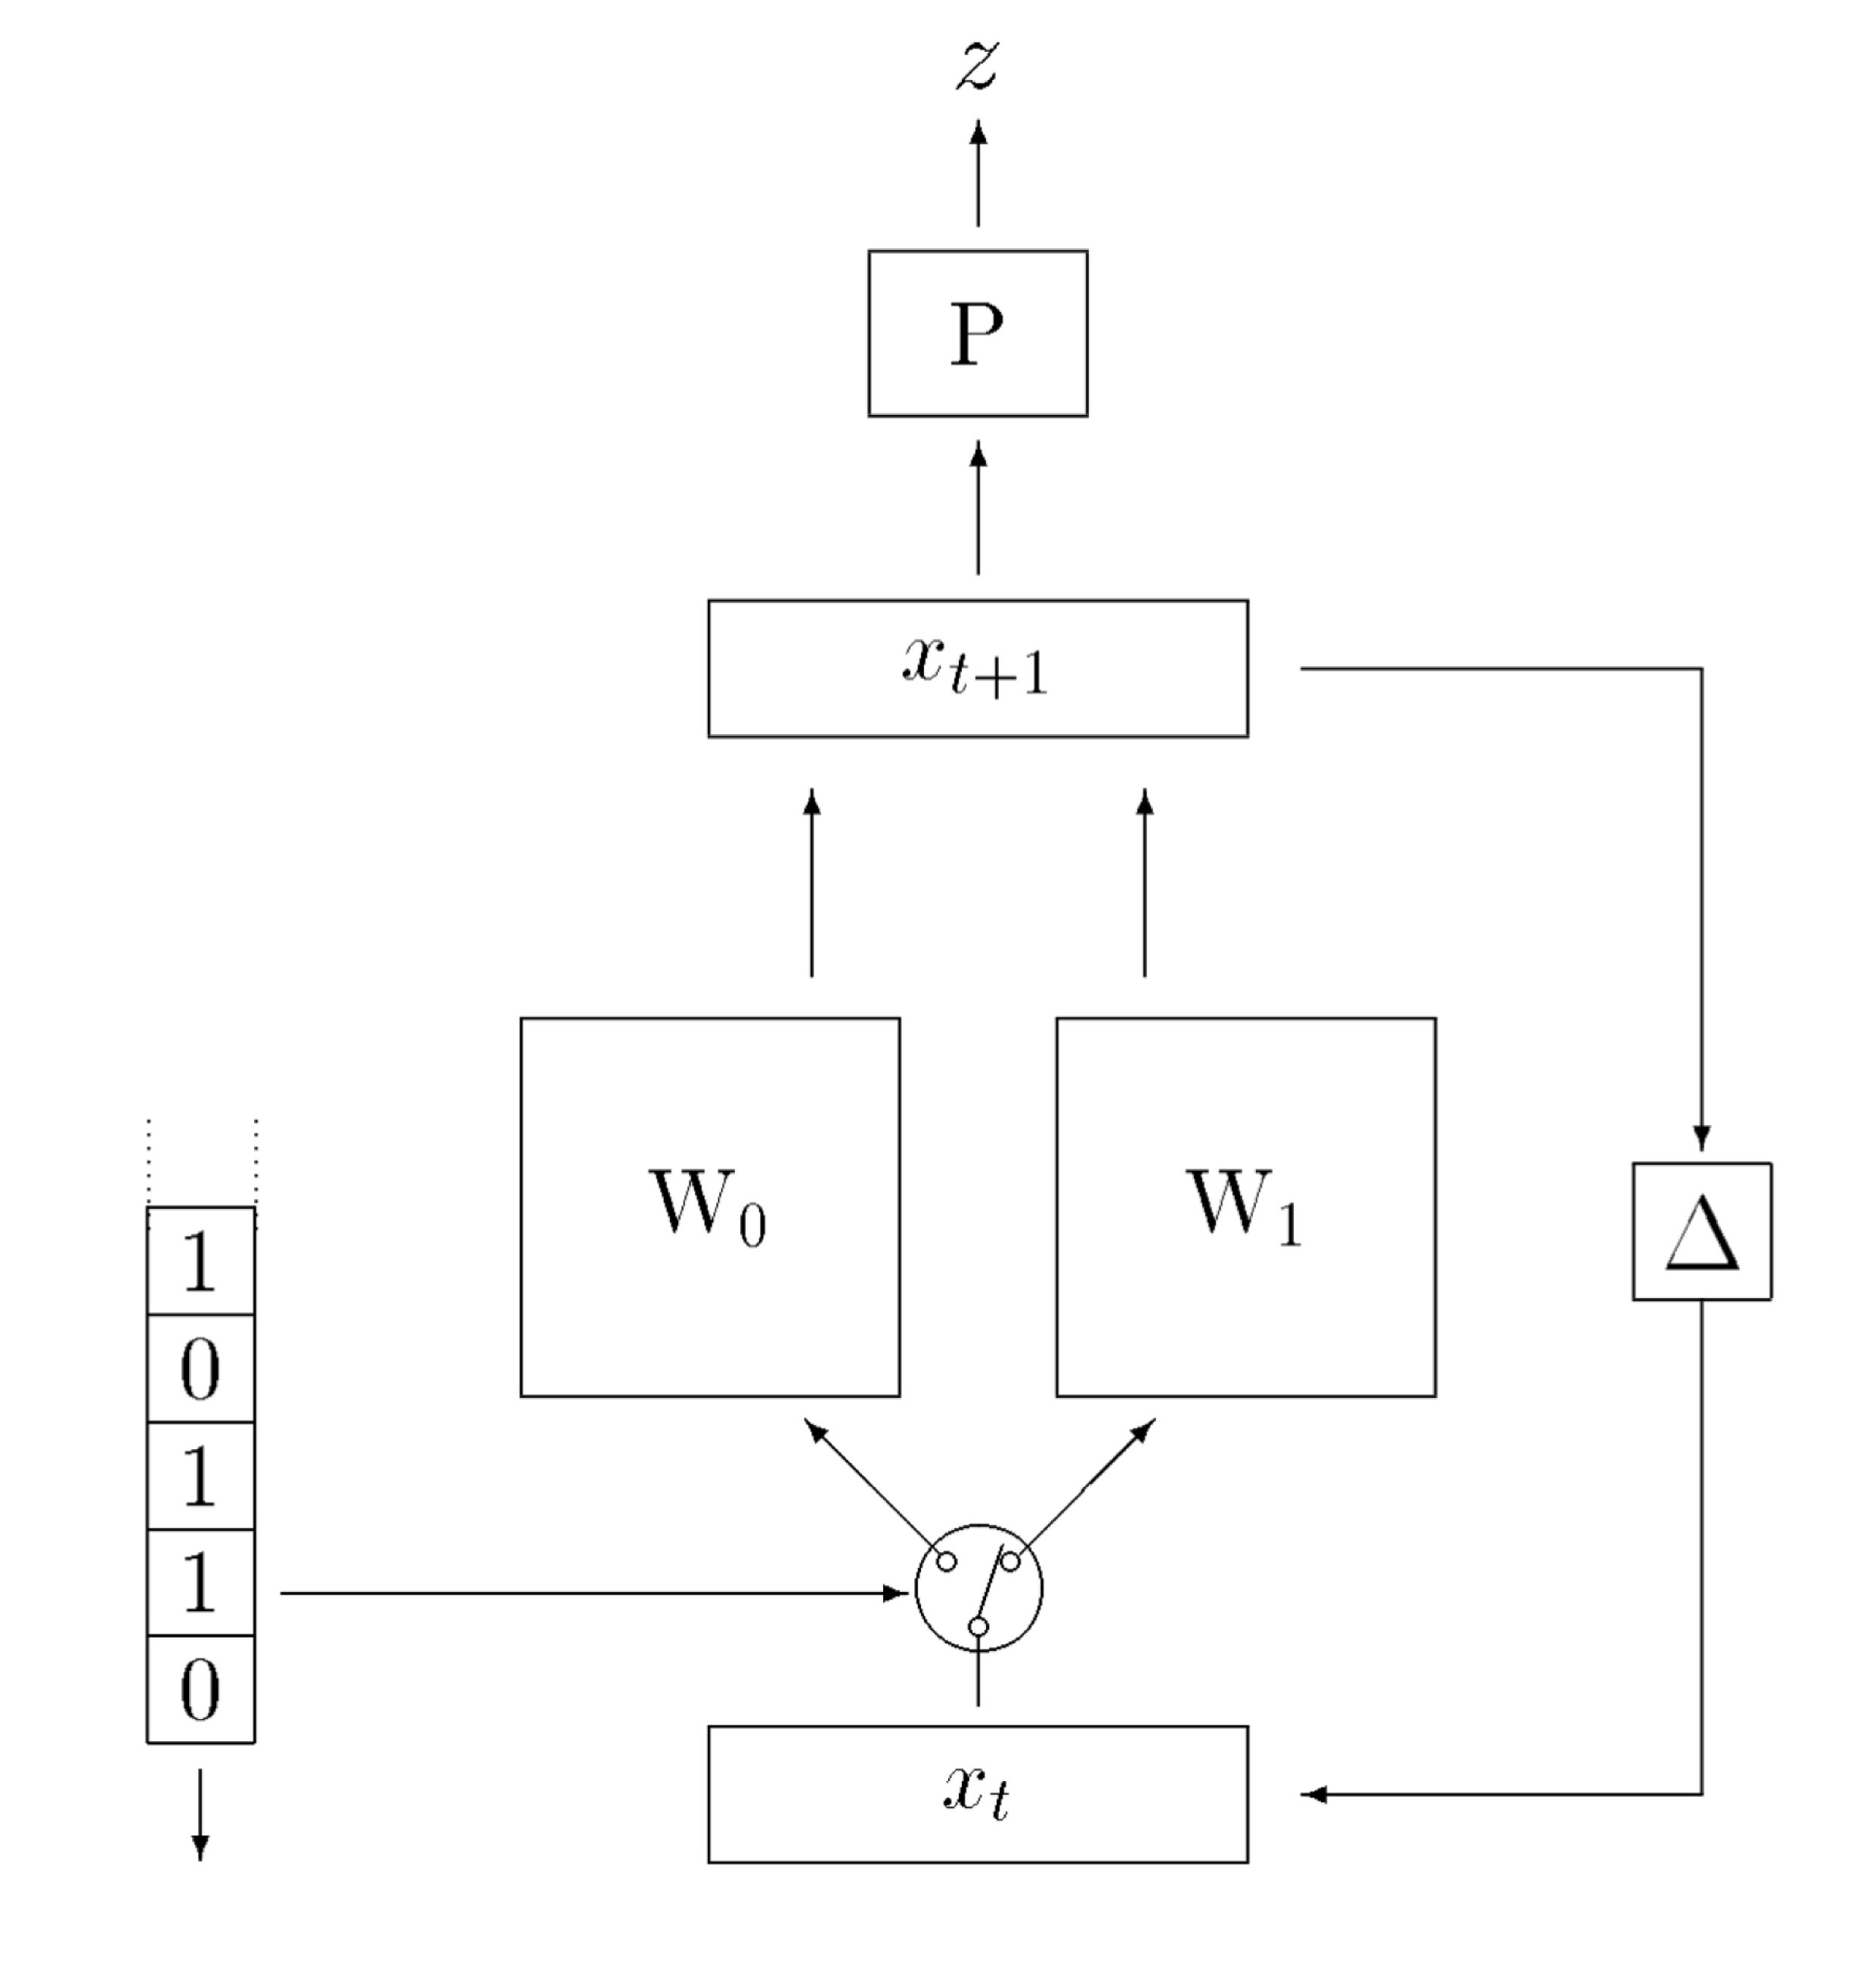
\includegraphics[width=12cm, height=8cm]{/home/noone/Documents/GitHub/neural_networks/out/images/recognisers_and_ports}
    \caption{}
    \label{fig: recognisers and ports}
\end{figure}

\section{Dynamical Recognizers}\label{sec:dynamical-recognizers}

    One common sequence processing task is Formal Language Recognition.
The network scans a sequence of characters one at a time, and must then output
either $1$ or $0$, in order to classify the sequence as Accept or Reject, respectively.
Consider, for example, this set of training data:

\begin{center}
\begin{tabular}{ |c|c|c| }
 \hline
 Accept & Reject \\
 1 & 0 \\
 11 & 10 \\
 111 & 01 \\
 1111 & 00 \\
 11111 & 011 \\
 111111 & 110 \\
 1111111 & 11111110\\
 11111111 & 10111111\\
 \hline
\end{tabular}
\end{center}

The natural generalisation from these data is to classify strings consisting entirely of $1$s as Accept and any string containing 000 as Reject.
This diagram shows the result of training a Second Order Network on these data.
The cross indicates the initial state while the dots indicate all the hidden states which occur while the network is processing a set of randomly generated test strings.
The dividing line shows the boundary between final states for which the string is classified as Accept, and those for which it is classified as Reject.

\begin{figure}[h]
    \centering
    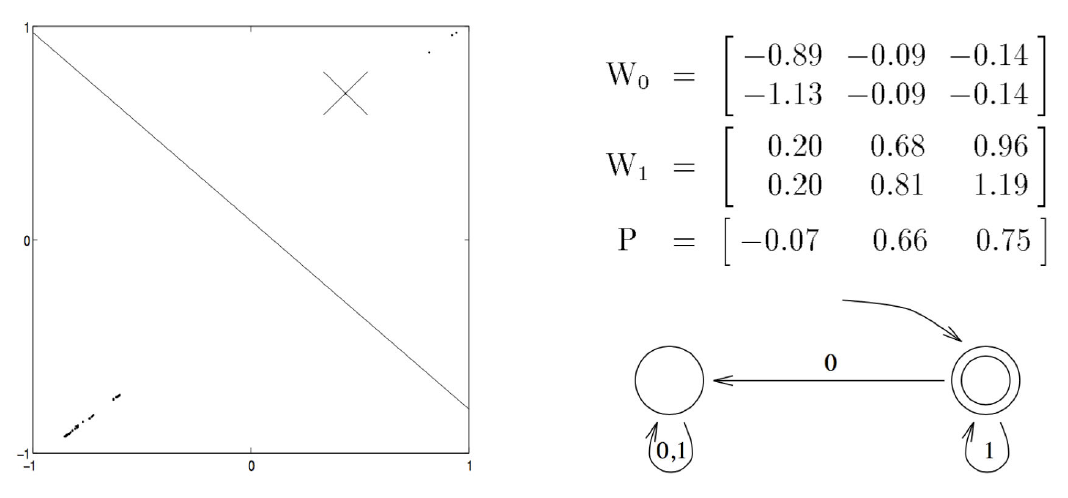
\includegraphics[width=12cm, height=8cm]{/home/noone/Documents/GitHub/neural_networks/out/images/dynamic-recognisers}
    \caption{}
    \label{fig: dynamic recognisers}
\end{figure}

In some cases, we can use analytical tools to extract a finite state machine which exactly mimics the behaviour of the network, as shown on the right for this example (Blair and Pollack, 1997).
Each cluster of hidden unit states is converted into a single state, the transitions between clusters are converted into arrows, and the initial state is indicated by an arrow with no origin.
The state(s) on the Accept side of the dividing line are indicated by a double circle;
those on the Reject side by a single circle.

Here is another example, where the network learns to Reject any string with three consecutive $0$s and Accept everything else.

\begin{center}
\begin{tabular}{ |c|c|c| }
 \hline
 cell1 & cell2 & cell3 \\
 cell4 & cell5 & cell6 \\
 cell7 & cell8 & cell9 \\
 \hline
\end{tabular}
\end{center}

\begin{figure}[h]
    \centering
    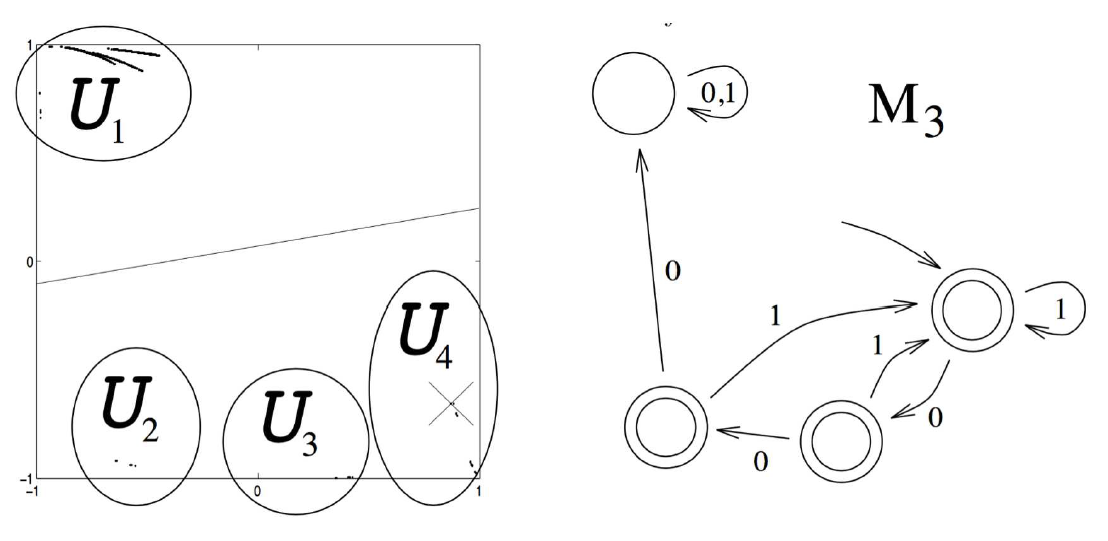
\includegraphics[width=12cm, height=10cm]{/home/noone/Documents/GitHub/neural_networks/out/images/dynamic-recognisers-2}
    \caption{dynamic recognisers 2}
    \label{fig: dynamic recognisers 2}
\end{figure}

In some cases, we can use analytical tools to extract a finite state machine which exactly mimics the behaviour of the network, as shown on the right for this example (Blair and Pollack, 1997).
Each cluster of hidden unit states is converted into a single state, the transitions between clusters are converted into arrows, and the initial state is indicated by an arrow with no origin.
The state(s) on the Accept side of the dividing line are indicated by a double circle;
those on the Reject side by a single circle.

Here is another example, where the network learns to Reject any string with three consecutive $0$s and Accept everything else.

\begin{center}
\begin{tabular}{ |c|c|c| }
 \hline
 Accept & Reject \\
 1 & 000 \\
 0 & 11000 \\
 10 & 0001 \\
 01 & 000000000 \\
 00 & 11111000011 \\
 100100 & 11111000011 \\
 001111110100 & 1101010000010111 \\
 0100100100 & 1010010001 \\
 0100100100 & 0000 \\
 11100 & 00000 \\
 \hline
\end{tabular}
\end{center}

\begin{figure}[h]
    \centering
    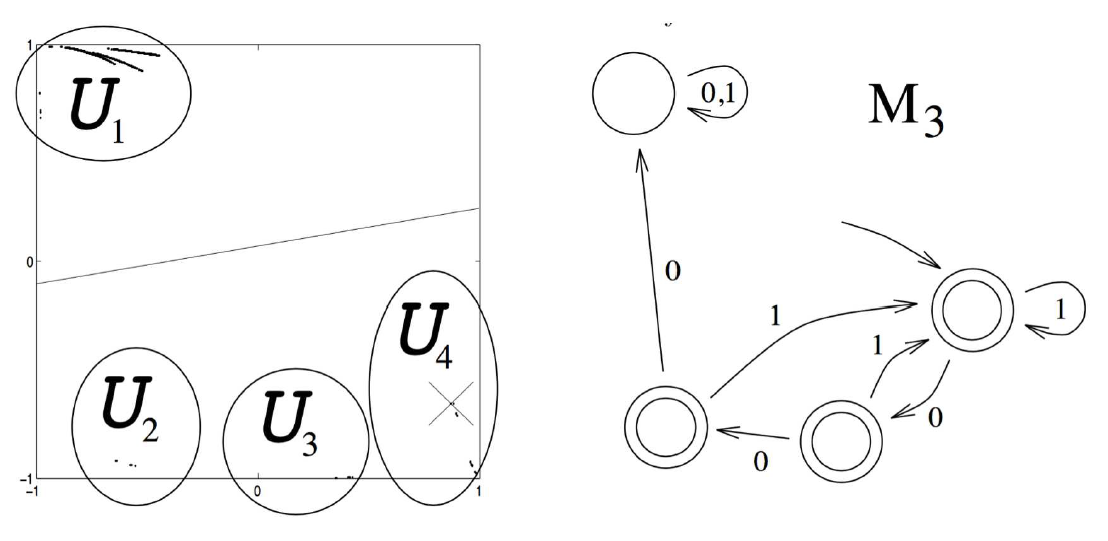
\includegraphics[width=12cm, height=8cm]{/home/noone/Documents/GitHub/neural_networks/out/images/dynamic-recognisers-4}
    \caption[dynamic recognisers 4]{dynamic recognisers 4}
    \label{fig: dynamic recognisers 4}
\end{figure}


\section{Non-Regular languages}\label{sec:non-regular-languages}

    Languages which can be characterized by a finite state machine are called Regular languages.
One simple example of a non-Regular language is $a^n b^n$ which means that every sequence of consecutive $a$s must be followed by an equal number of consecutive $b$s −-− for example:

abaabbabaaabbbaaaabbbbabaabbaaaaabbbbb. . .

A SRN with 2 inputs, 2 hidden nodes and 2 outputs can be trained to predict the $a^n b^n$ language (Wiles and Elman, 1995).
In this case, the network must scan a sequence of input characters one at a time, and try at each step to predict the next character in the sequence.
In some cases, the prediction is probabilistic.
For the $a^n b^n$ task, the first $b$ is not predictable, but subsequent $b$ and the initial $a$ in the next subsequence are predictable.

    \begin{figure}[h]
    \centering
    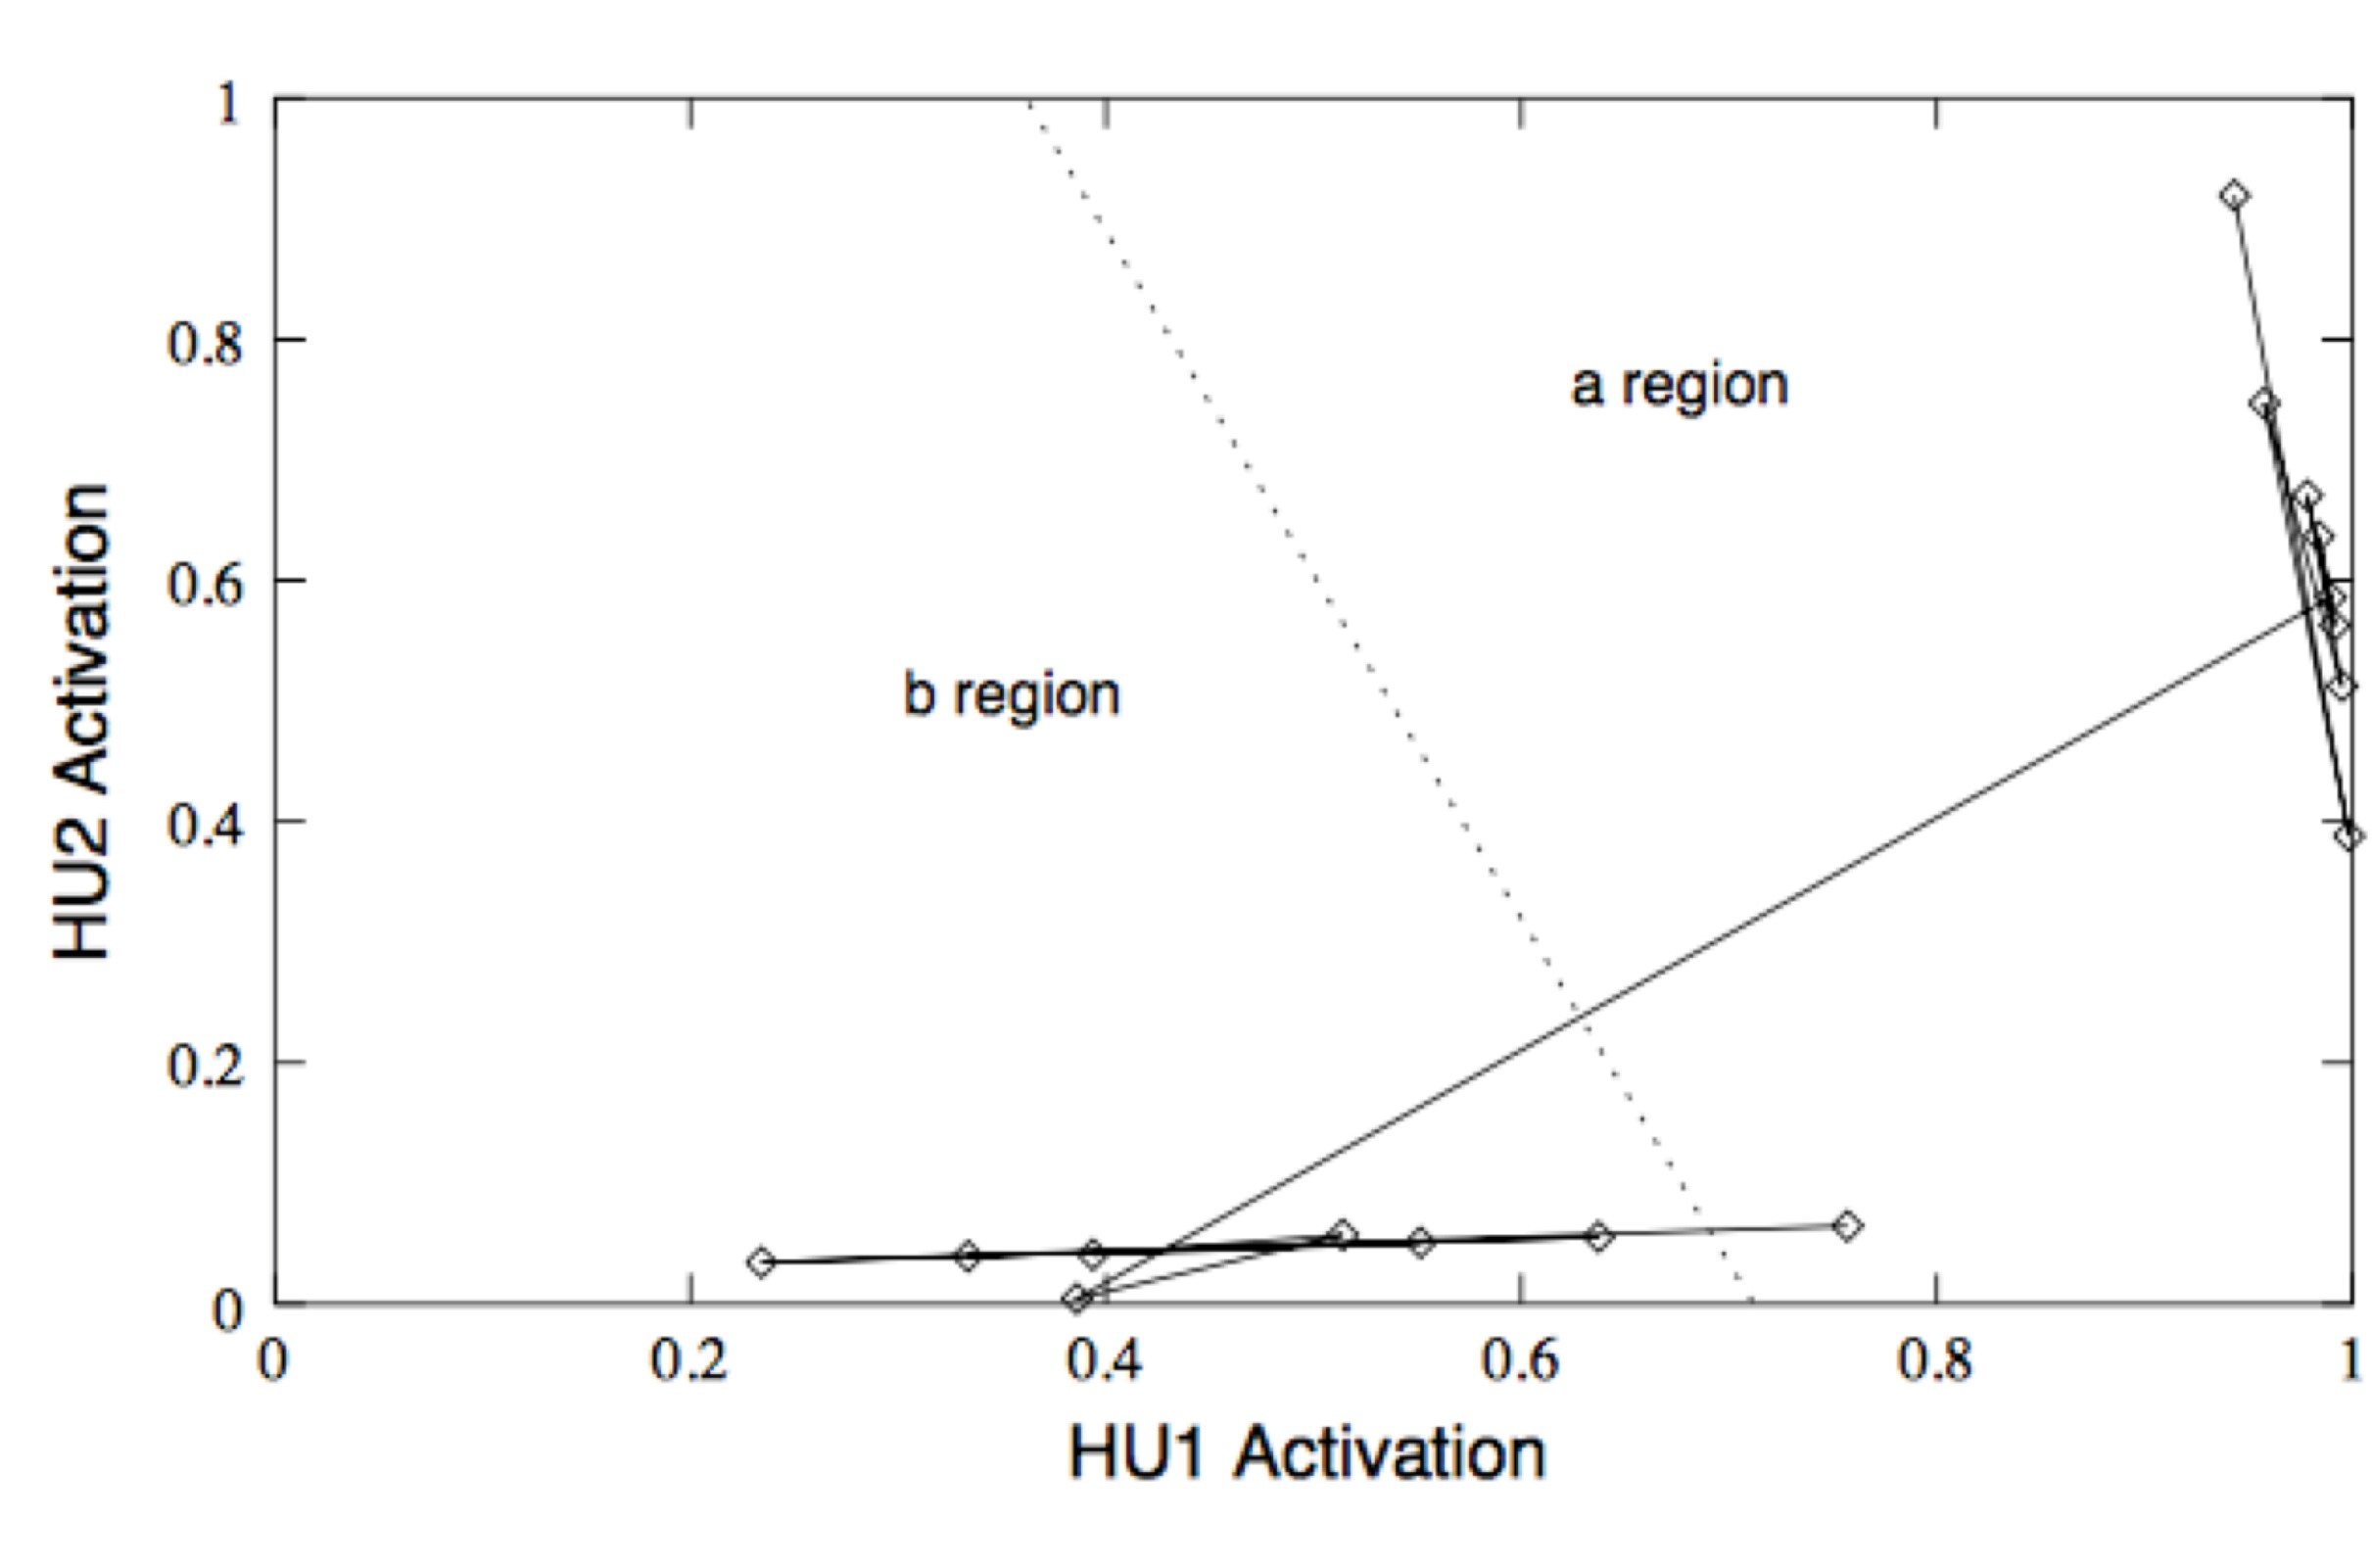
\includegraphics[width=12cm, height=8cm]{/home/noone/Documents/GitHub/neural_networks/out/images/non-regular-languages}
    \caption[non-regular languages]{non-regular languages}
    \label{fig: non-regular languages}
    \end{figure}

The network does not implement a Finite State Machine but instead makes use of two fixed points in activation space ––– one attracting, the other repelling (Wiles and Elman, 1995).
The network effectively *counts up* the $a$s as it oscillates towards the attractive fixed point and then counts down the same number of bbb's as it oscillates away from the repelling fixed point.
When the recurrent mapping is linearised at the two fixed points we find that the two major eigenvalues are nearly reciprocal to each other.
Interestingly, networks trained only up to $a^{10} b^{10}$ can often generalise up to $a^{12}b^{12}$.

Training the weights by evolution is more stable than by backpropagation.
Networks trained by evolution sometimes exhibit monotonic rather than oscillating trajectories.

\begin{figure}[h]
    \centering
    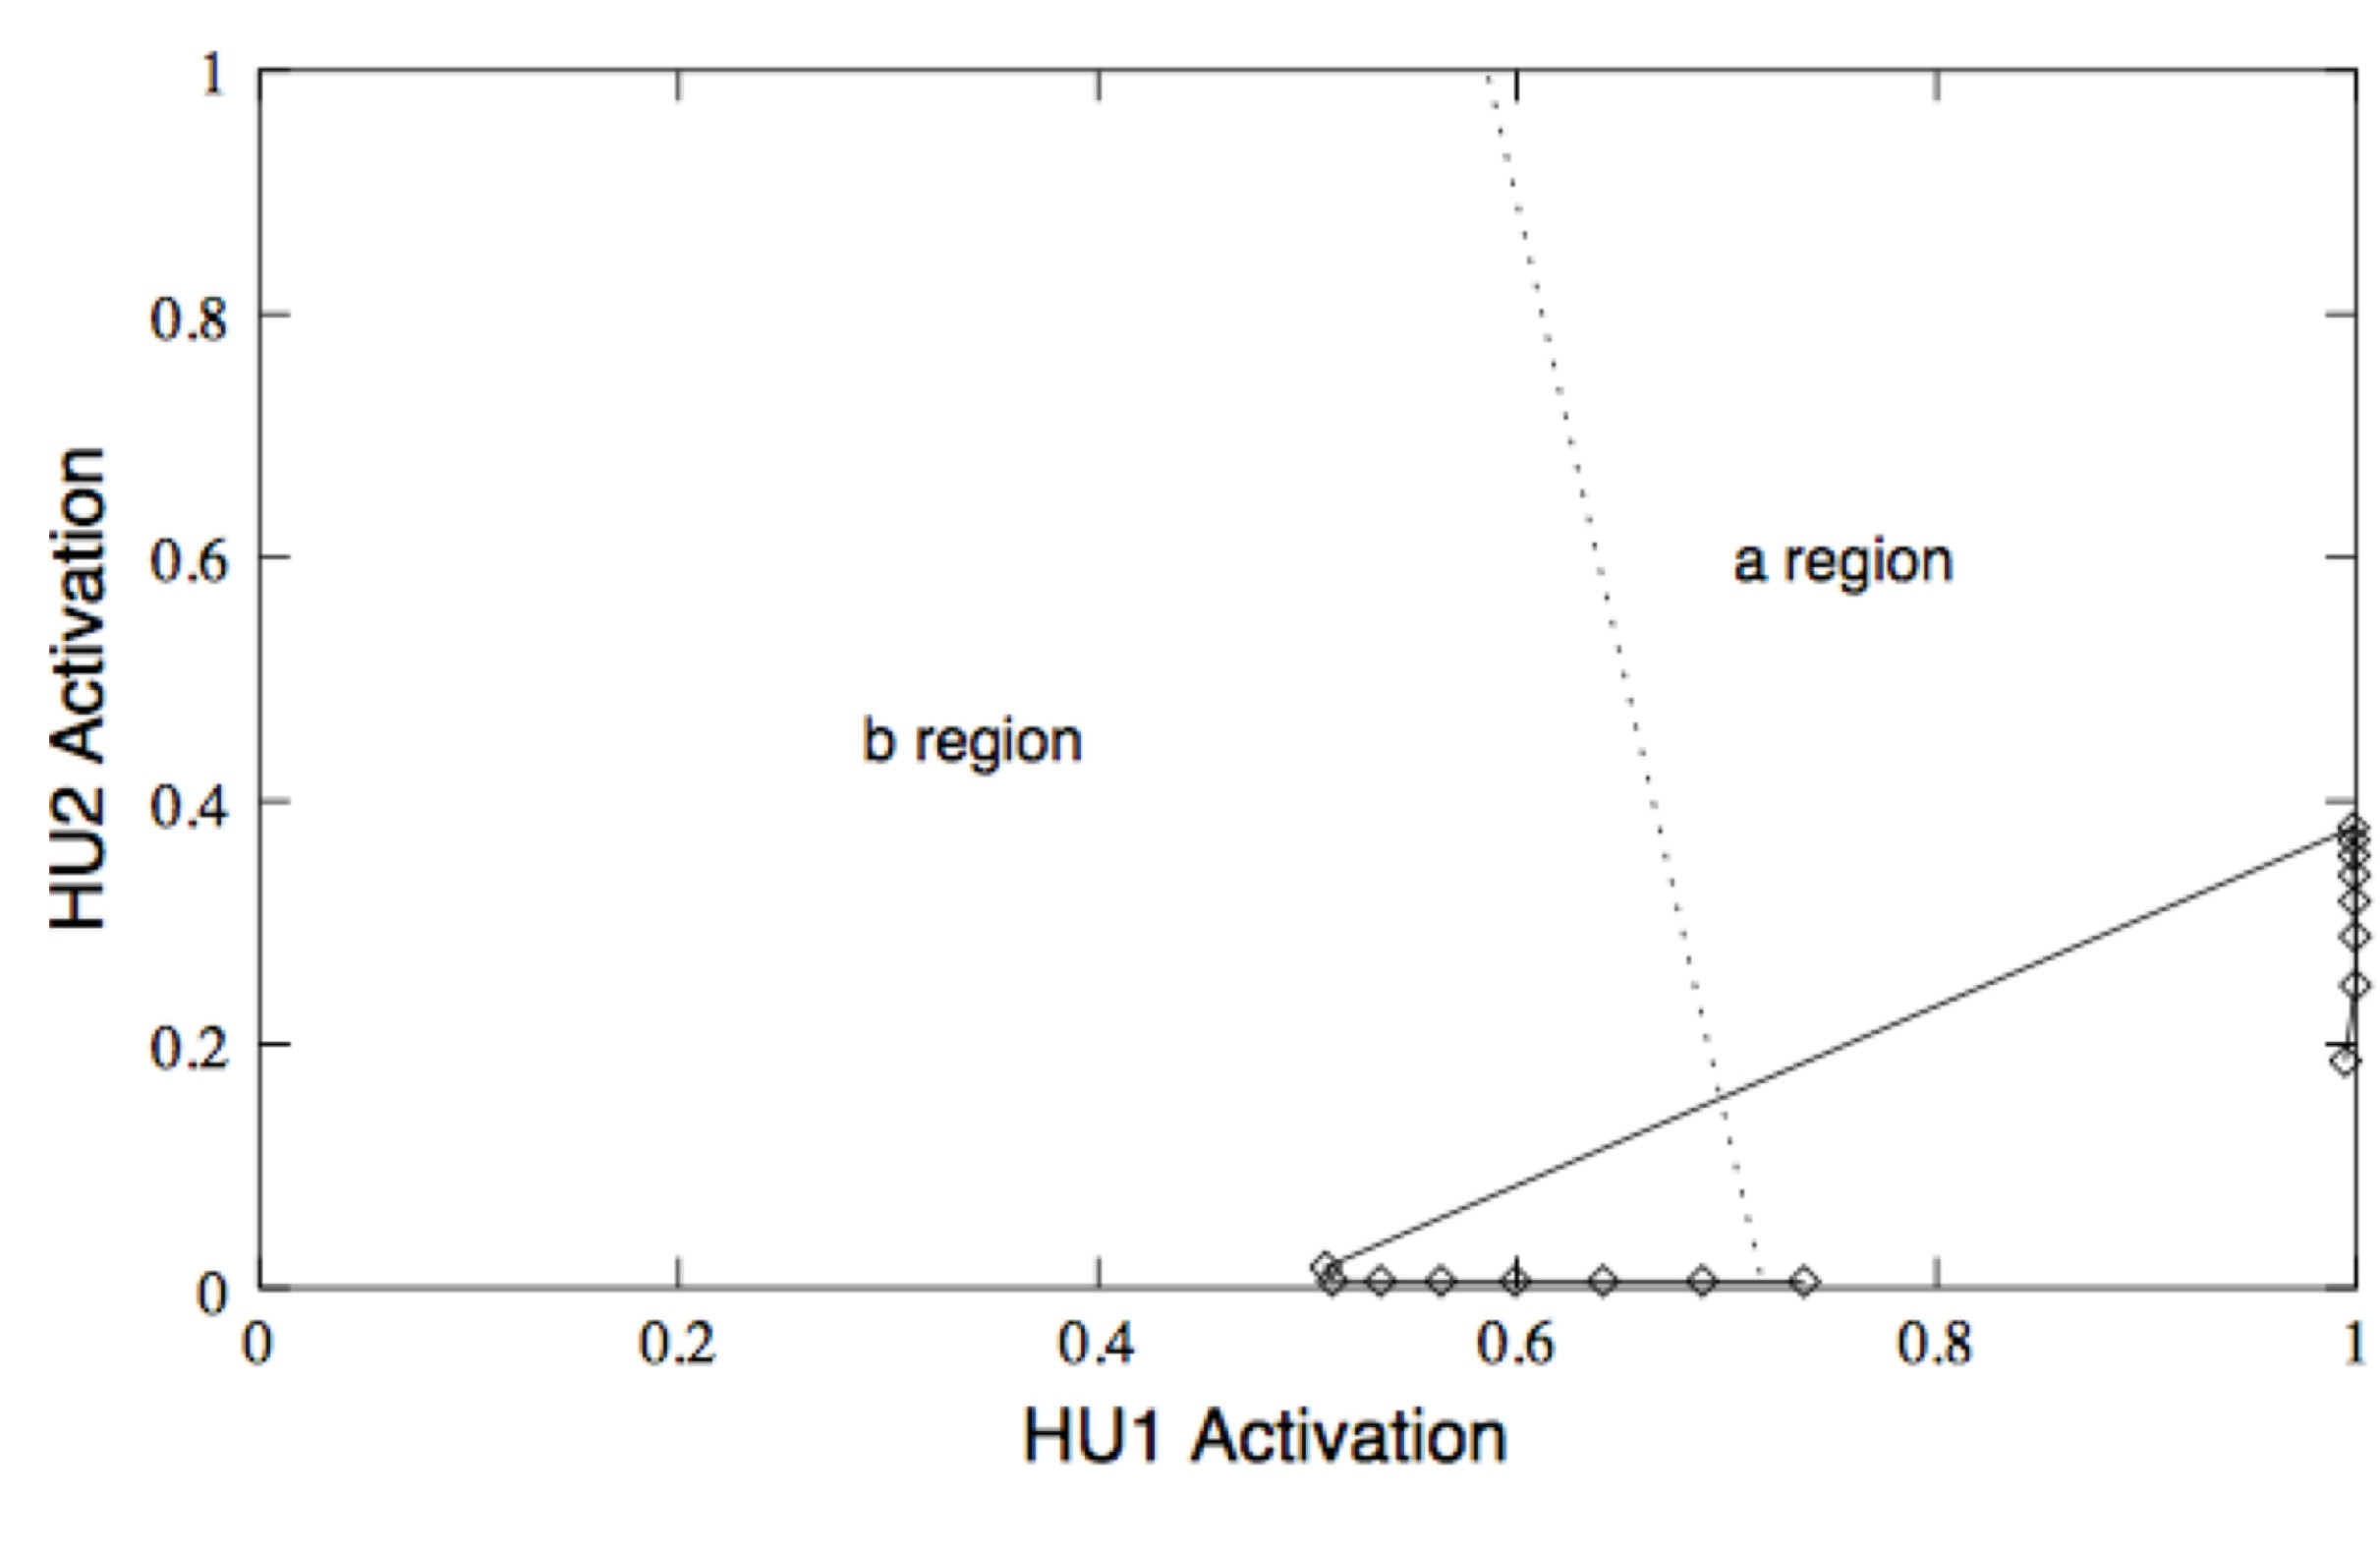
\includegraphics[width=12cm, height=8cm]{/home/noone/Documents/GitHub/neural_networks/out/images/non-regular-languages-2}
    \caption[non-regular languages 2]{non-regular languages 2}
    \label{fig: non-regular languages 2}
\end{figure}

\section{Counting by spiralling}\label{sec:counting-by-spiralling}

    SRN's can also be trained to recognise the balanced bracket language, treating aaa as open bracket and bbb as close bracket (Boden, 2003).
In this case, the eigenvalues of the linearised mapping at the fixed points are complex numbers, and the network counts up the $a$s by spiralling inwards towards a fixed point and counts down the $b$s by spiralling outwards.

\begin{figure}[Hh]
    \centering
    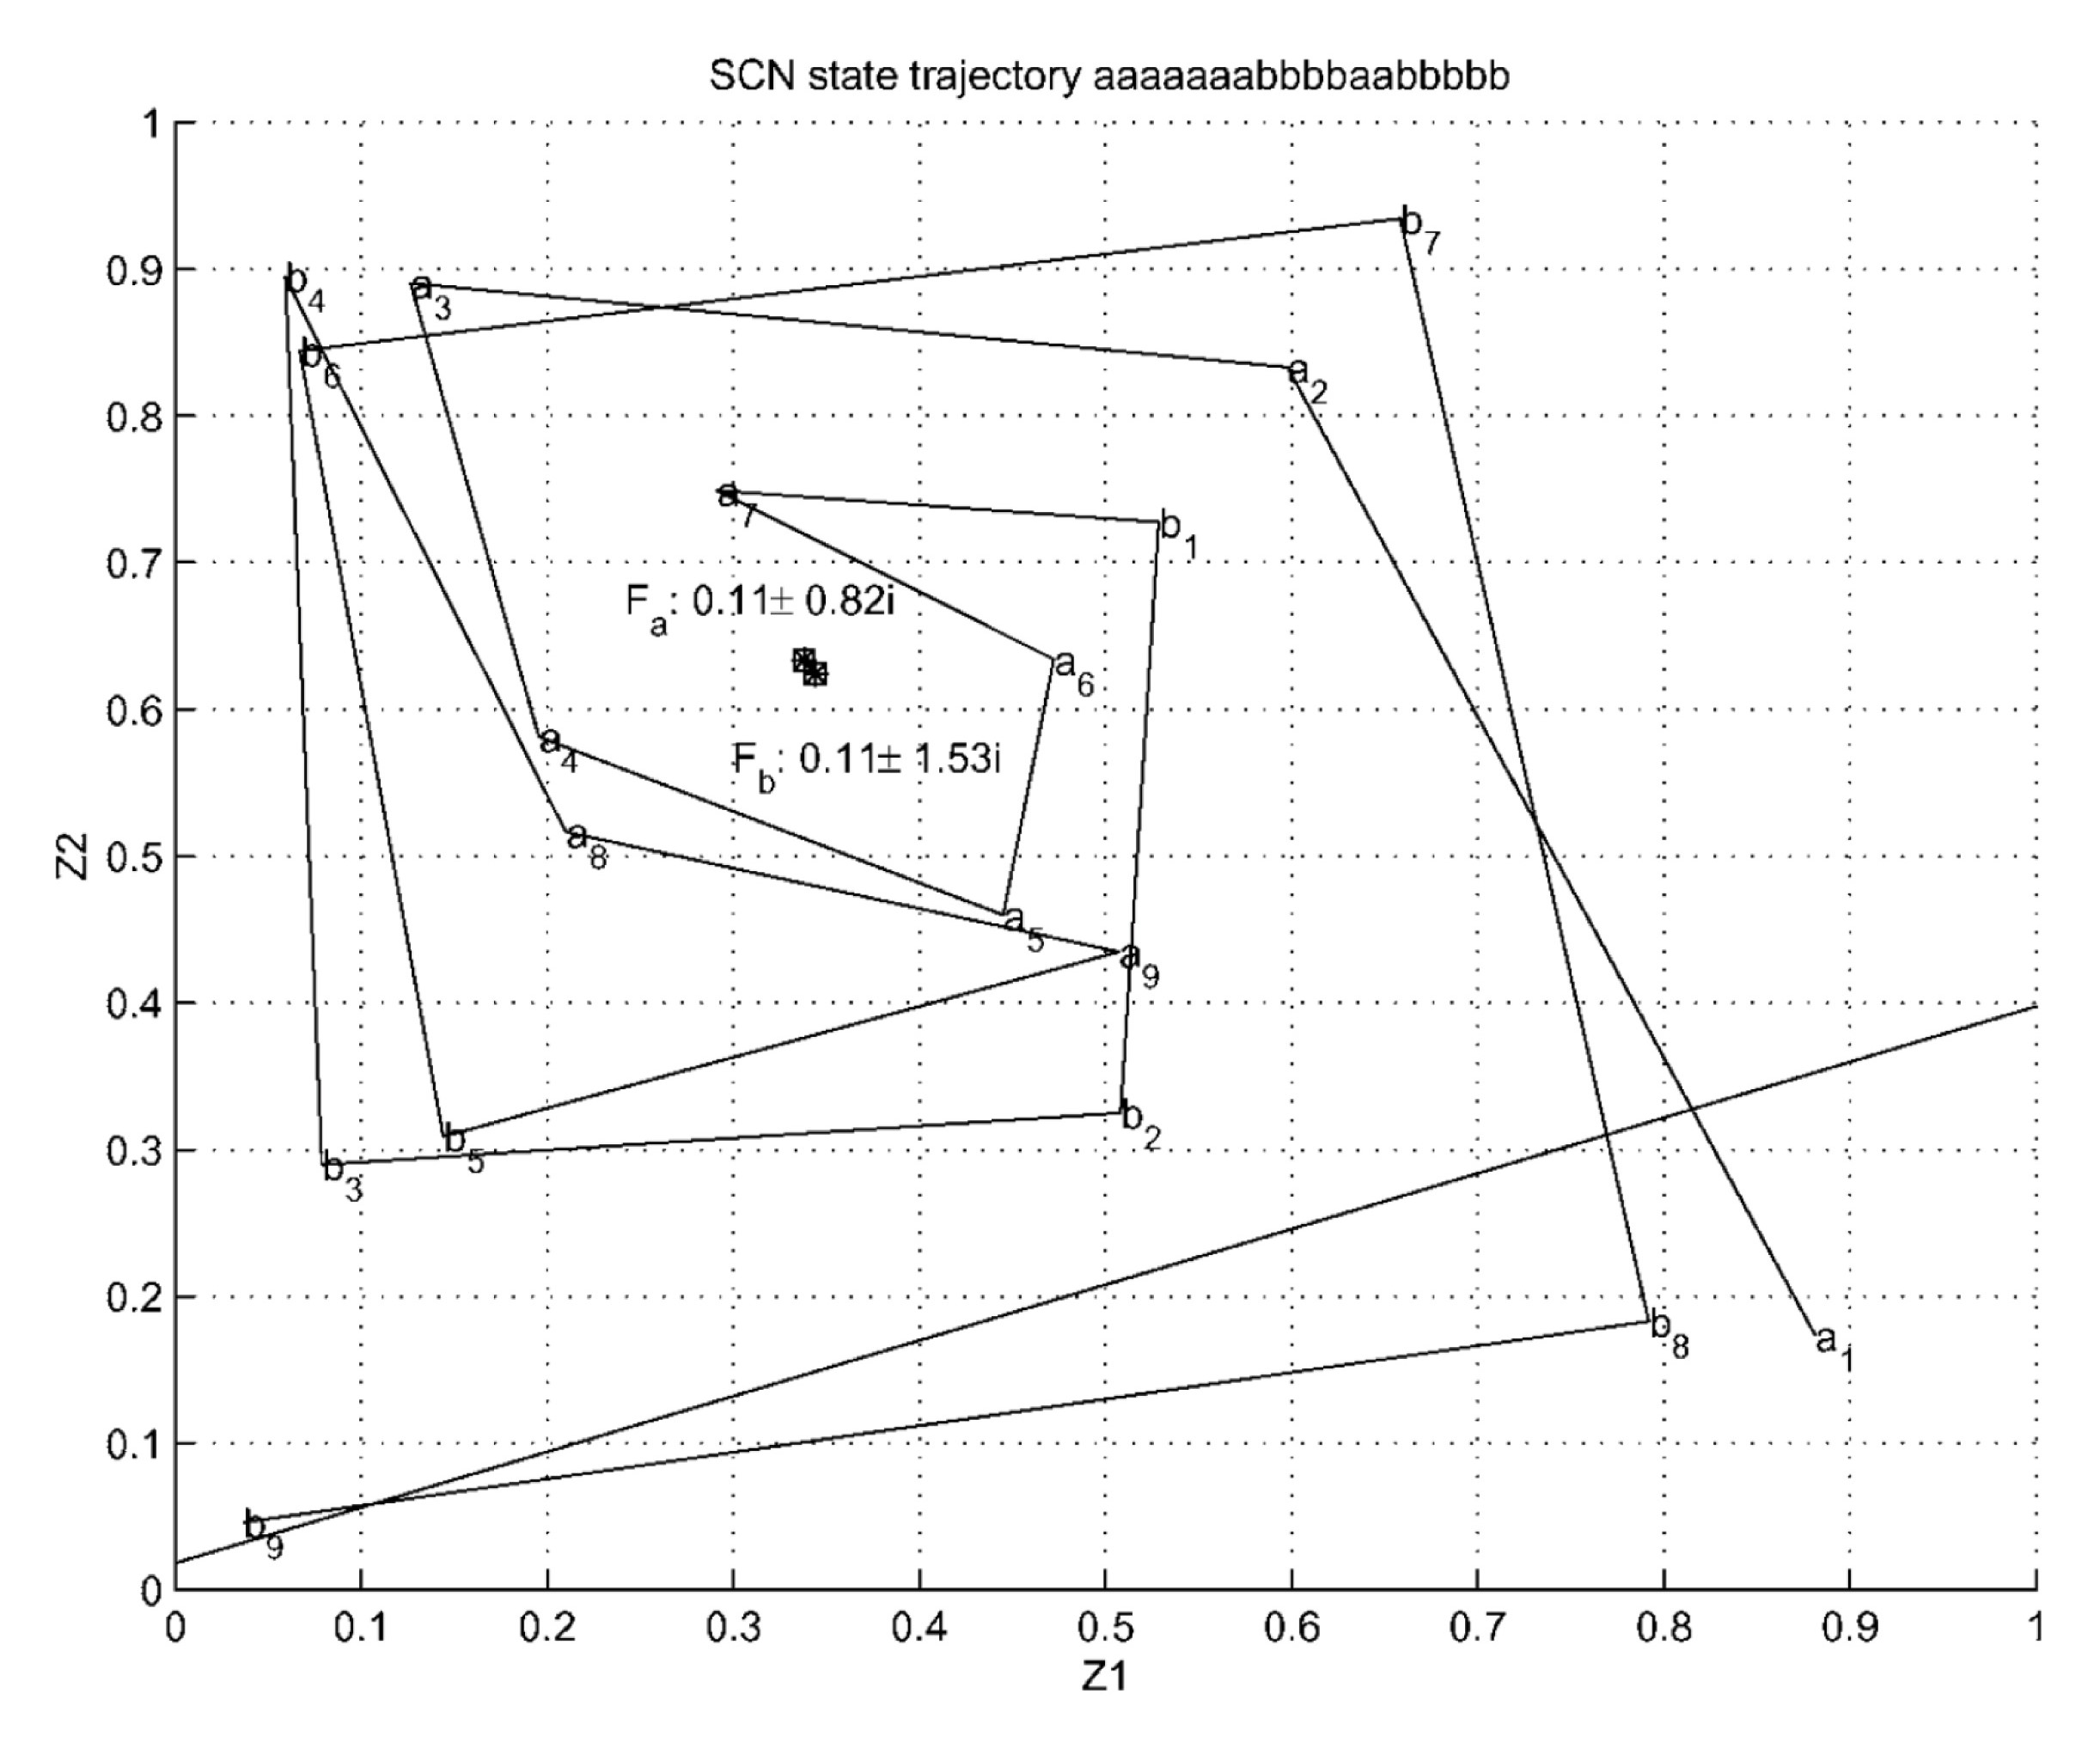
\includegraphics[width=12cm, height=8cm]{/home/noone/Documents/GitHub/neural_networks/out/images/counting-by-spiralling}
    \caption[counting by spiralling]{counting by spiralling}
    \label{fig: counting by spiralling}
\end{figure}

    \section{Hidden Uni Dynamics for $a^n b^n c^n$}\label{sec:hidden-uni-dynamics-for-$a^n-b^n-c^n$}

An SRN with three inputs, three hidden units and three outputs can be used to learn the language $a^n b^n c^n$ which is classified as Mildly Context Sensitive (Chalup, 2003).
The network counts down in one direction while simultaneously counting up in another direction, thus producing a star-shaped pattern.

\begin{figure}[h]
    \centering
    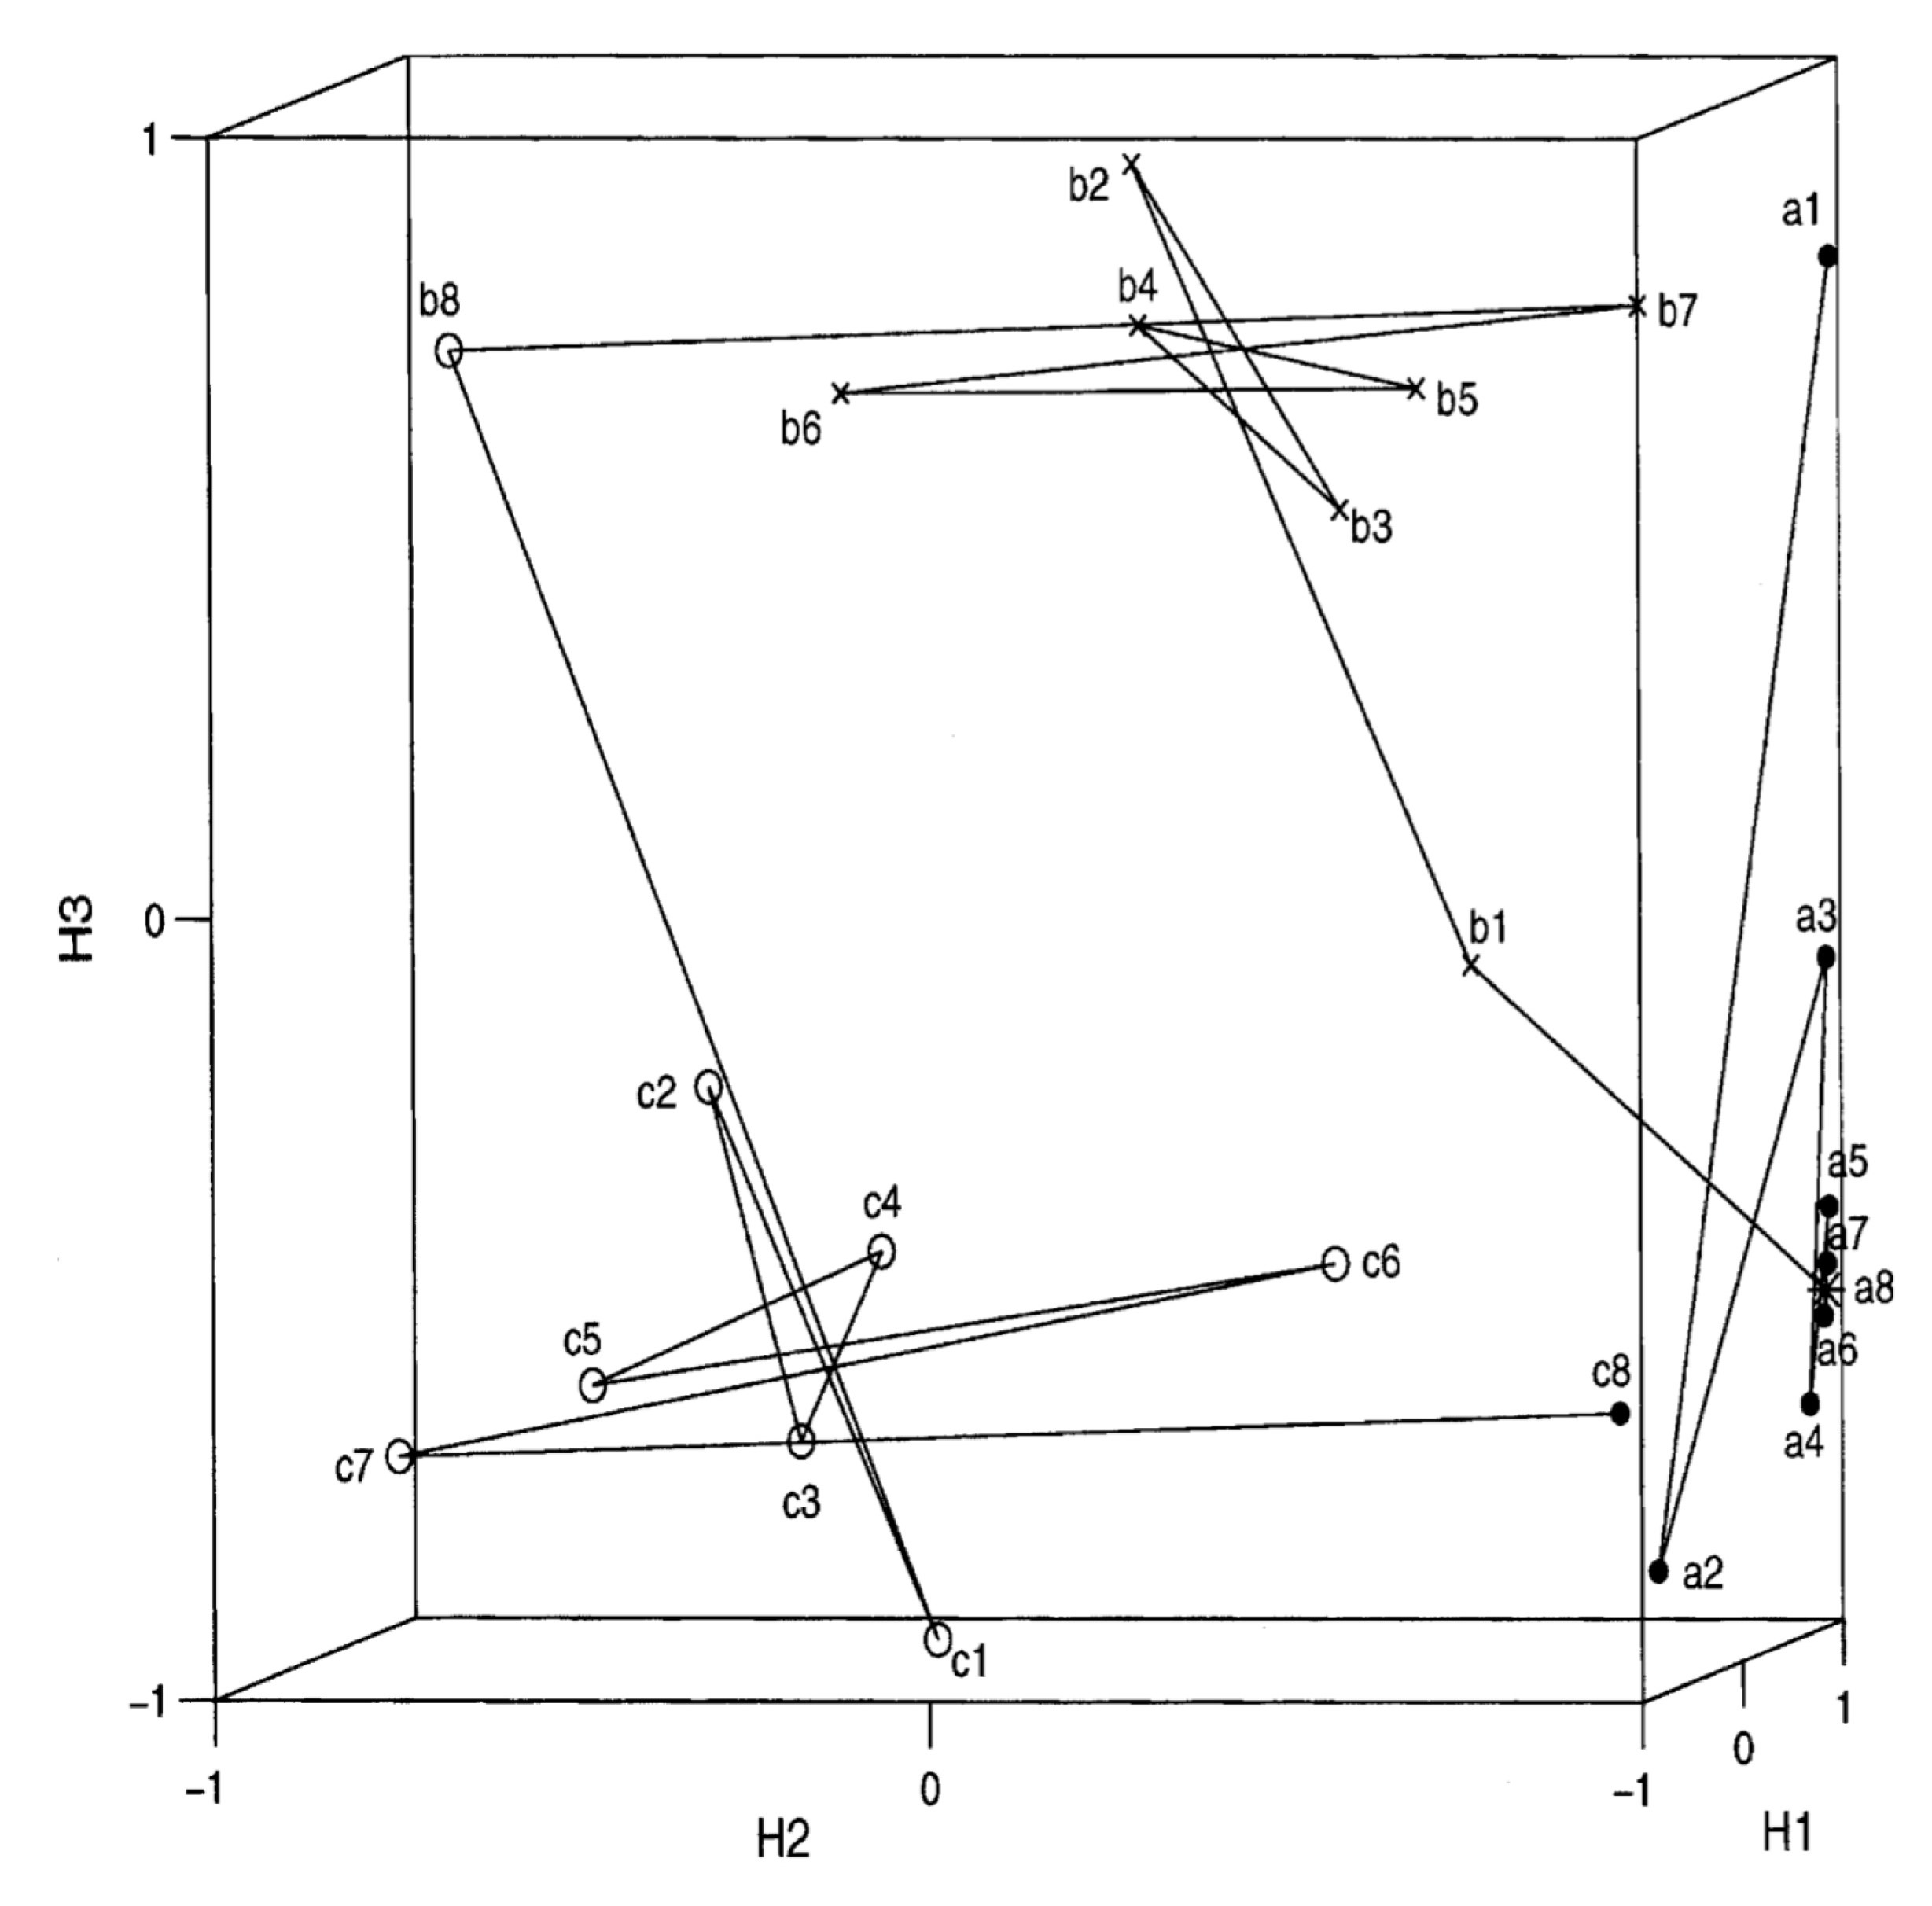
\includegraphics[width=12cm, height=8cm]{/home/noone/Documents/GitHub/neural_networks/out/images/hidden-unit-dynamics}
    \caption[hidden unit dynamics]{hidden unit dynamics}
    \label{fig: hidden unit dynamics}
\end{figure}

This analysis of network dynamics with simple languages is illuminating.
But, in the end, SRNs are limited in the range of dependencies they are able to learn, for reasons analogous to the vanishing gradient problem which we discussed in Week 2 in the context of feedforward networks.
In the next section we will introduce Long Short Term Memory, which is able to learn longer range dependencies and $-$ in combination with word vectors, attention and other enhancements $-$ can perform serious real world tasks such as multilingual translation.

insert video

\end{document}